\section{Pipeline}
The pipeline was constructed to formalize and automatize the process of data preparation for the neural networks.
It was written in Snakemake workflow management system \cite{koster2012snakemake}, which is highly popular in the bioinformatics field with approximately 3 new citations each week.
The workflows consists of rules, which define the data dependency in form of rule input files, rule output files and the script, which needs to be executed to get from input to output. 
This definitions make using of Snakemake very convenient.
The rules are defined as a subset of YAML, extended by the option to run python code directly.
This makes them easily readable by humans.
The structuring of the workflow allows seamless scalability to server environments and parallelization to multiple cluster nodes and multiple cores.
This capability was very crucial for this project due to the amount of data available.
Furthermore, Snakemake automatically checks for completed rules, which is in turn used to run only the rules needed for the defined target.
It also check the exit code of the scripts and informs user if there is an error during the execution and therefore decreases a chance of working with faulty data to the minimum.
Finally, conda \cite{conda}, the package management system, is nicely integrated into Snakemake, which simplifies the installation of most packages and bioinformatics tools needed during the analysis.
It is also possible to fix package versions used during the analysis, which hugely improves reproducibility.
Next, we present the main steps in the pipeline.
The complete pipeline can be found on our GitHub repository \cite{github}.

\subsection{PSI-BLAST}
The first step in the pipeline was the construction of the PSSMs of the protein sequences.
For this purpose, we used the PSI-BLAST \cite{altschul1997gapped}, an improved variation of the BLAST algorithm focused on PSSM construction.
The PSI-BLAST first identifies proteins similar to our query protein from the database above a certain threshold.
The threshold is inversely proportional to an E-value, which represents the number of expected hits in a database of a particular size just by random chance.
In our project, we used a default E-value of 10.
The proteins identified as similar are then aligned to the query protein.
Proteins with an insufficient alignment score are discarded from the set of similar proteins.
Here, the parameter \textbf{-inclusion\_ethresh} is used to determine which alignments should be included in the set. 
Afterwards, the MSA is constructed from the set of similar proteins and the PSSM profile is calculated from this MSA.
The PSSM profile is then used to identify proteins corresponding to this profile, in a similar fashion as the original sequence was used.
A new PSSM profile is then calculated using these newly identified proteins.
This process is iterated multiple times, improving the PSSM each iteration as was shown in Altschul et al. \cite{altschul1997gapped}.
In our implementation, we used 3 iterations to construct the final PSSM. 
The PSI-BLAST algorithm is sketched out in Figure \ref{fig:psi_blast}
\begin{figure}
    \centering
    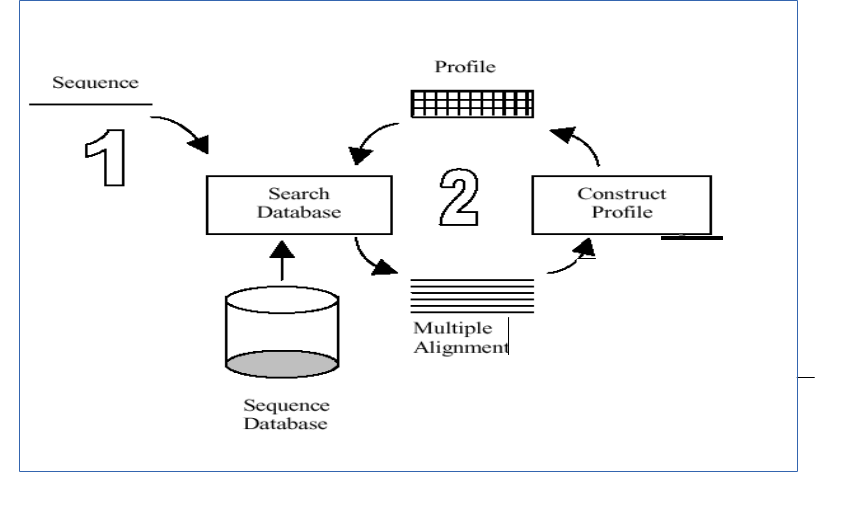
\includegraphics[width=\linewidth]{imgs_andy/psi_blast.png}
    \caption{PSI-BLAST process}
    \label{fig:psi_blast}
\end{figure}

% https://www.youtube.com/watch?v=IXuzKjCm0ME seems like a good source

\subsection{HHblits}
Another step, parallel with the PSI-BLAST step was construction of MSA using HHblits \cite{remmert2012hhblits}.
This MSA was later used as an input to the Potts models.
The HHblits takes slightly different approach to MSA construction than the PSI-BLAST, which we considered an advantage, because the correlation of the input features to the neural networks was decreased.
The HHblits first converts the query sequence to a Hidden Markov Model (HMM).
This query HMM is then compared to HMMs from the database.
The database HMMs below a certain E-value threshold are then added to the query MSA, from which a query HMM for the next iteration is constructed.
This process is then repeated defined number of times.
In this project, we used E-value of 0.001 and 3 iterations to arrive at the final MSA.

\subsection{plmc}
To create a Potts models from the MSA, we used a plmc software from Debora Marks Lab \cite{plmc}.
Given the MSA in FASTA format, this software produced the Potts models pairwise interactions $J$ values and the propensities $h$.
Furthermore, we extracted Frobenius norm of the pairwise interactions.
The plmc software used the second order optimization algorithm LBFG-S to iteratively fit these parameters.
The number of maximum iterations used in our pipeline was 500.
% \cite{potts1}???

\subsection{input creation}
The last step of the input preparation pipeline was to create an input tensor for the neural networks.
We used the input tensor of size $L \times L \times C$, where $L$ is the length of the protein sequence and $C$ is the number of channels.
To create such tensor, we used the Potts model parameters, one-hot encoded protein sequence and the PSSM profile.
We also added channels representing positions and the length of the protein.
The complete description of the input tensor was as follows.

\begin{itemize}
    \item Potts model's pairwise interactions $J$ transformed from size $L \times L \times 21 \times 21$ to $L \times L \times 441$
    \item Frobenius norm of pairwise interactions $J$ of size $L \times L \times 1$
    \item positions from $0$ to $L-1$ transformed from size $L \times 1$ to $L \times L \times 1$
    \item Potts model's propensities $h$ transformed from size $L \times 21$ to $L \times L \times 21$
    \item one-hot encoded protein sequence transformed from size $L \times 21$ to $L \times L \times 21$
    \item PSSM profile transformed from size $L \times 20$ to $L \times L \times 20$
    \item tensor of size $L \times L \times 1$ containing a constant value of protein length
\end{itemize}

The positions, Potts model's propensities $h$, one-hot encoded protein sequence and PSSM profile were simply repeated $L$ times along the axis to match the required size.
Both, repetition along the first and second axis, were used, therefore the resulting number of channels $C$ was $441 + 1 + 2 \cdot 1 + 2 \cdot 21 + 2 \cdot 21 + 2 \cdot 20 + 1 = 569$. 

\subsection{Output encoding}

The labels used for training were downloaded from the Protein Data Bank (PDB) which offers rich description of many proteins, including their tertiary structure. Domains with missing coordinates were filtered out of the dataset.
        
% For the reasons of structure realization and residue placement, AlphaFold (and also ProSPr) extracted the C$_\beta$ coordinates of the residues (C$_\alpha$ for glycine) \cite{alphafold}.

Although distance is a continuous measure, and it would make perfect sense to treat the problem as a regression one, AlphaFold discretized the distances into 64 bins ranging from 2 to 22\AA, with one bin used for distances larger than 22\AA and one bin for missing data (in our case a zero padding label). 
The reason for doing so becomes clearer after understanding of how the structure realization (the last step of the entire pipeline) was performed.

To make the task slightly simpler for the neural network, we binned the distances into 32 bins (with the first bin - bin 0 used for missing values / padding and last bin for distances larger than 22 \AA).
        
The secondary structure was classified into 9 categories (padding label + 8 DSSP classes) suggested by DSSP (Dictionary of Protein Secondary Structure) \cite{dssp1, dssp2, dssp3}.
The categories are shown in table \ref{tab:dssp0}.

On top of the secondary structure classification, the output of the DSSP program also conveniently includes the torsion angles $\phi$ and $\psi$. These were categorized to 37 bins (padding label + bin for every 10\degree).

\subsection{Data}

\subsubsection{CATH}
\begin{figure}
    \centering
    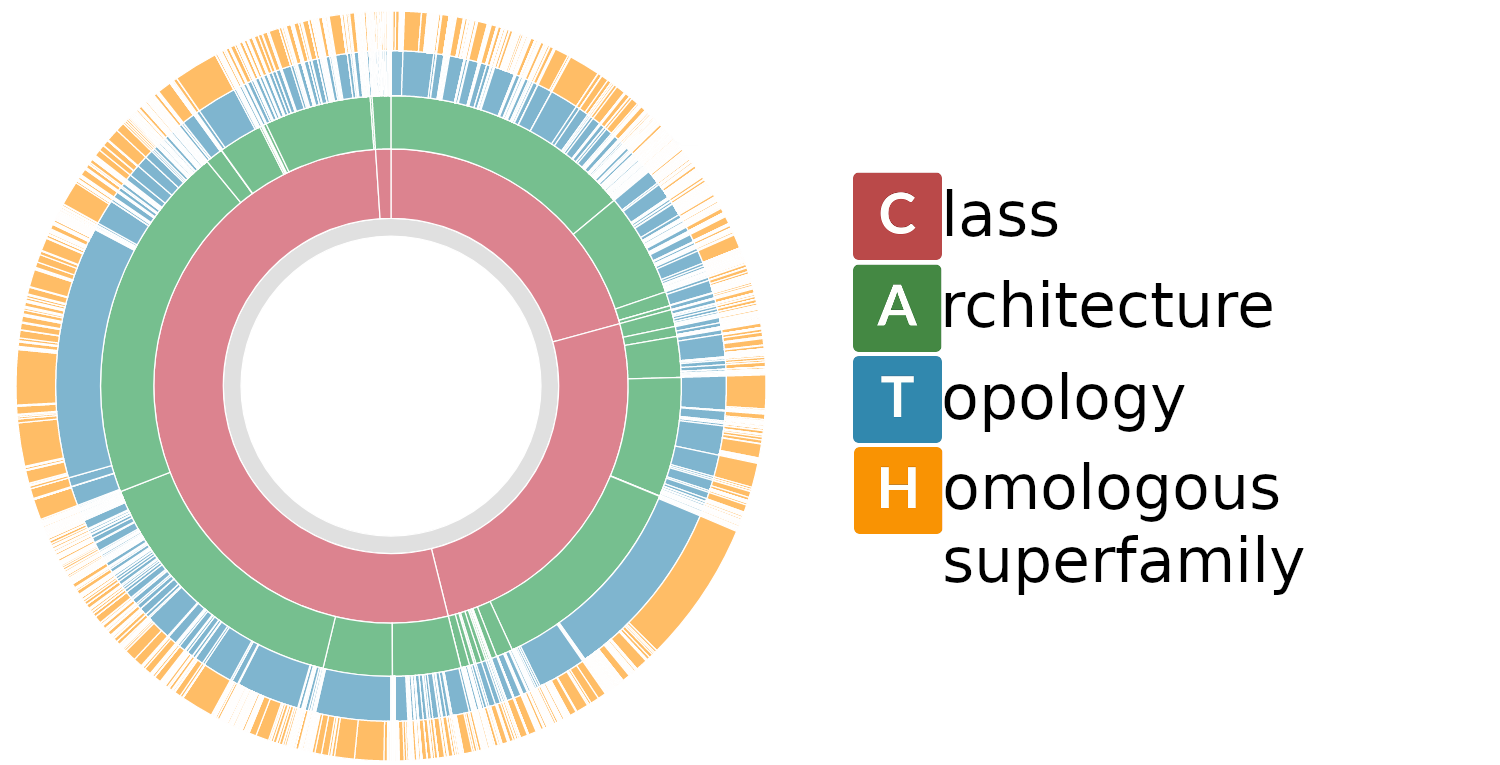
\includegraphics[width=\linewidth]{imgs_tomas/cath.png}
    \caption{CATH hierarchy \cite{cath}}
    \label{fig:cath}
\end{figure}

For training and evaluation of models, it is important to use diverse data sets, that capture a wide range of different scenarios and thus force the model to generalize well. For this reason a CATH dataset was created.
CATH is a database that clusters proteins with known structures based on 4 criteria: Class (secondary structure classes), Architecture (secondary structure arrangement in 3D space), Topology (how secondary structure elements are connected) and Homologous Superfamily (evolutionary relationship between domains). 
Figure \ref{fig:cath} shows the hierarchical relationship between the classes.
    
To ensure dataset diversity, we used a dataset of sequences with pairwise sequence similarity of at most 35\%. 
The list of domains together with their sequences in \texttt{fasta} format can be accessed at: \href{ftp://orengoftp.biochem.ucl.ac.uk/cath/releases/latest-release/sequence-data/cath-domain-seqs-S35.fa}{oregonftp.biochem.ucl.ac.uk}.
    
Domains are short regions of proteins that fold more or less independently of each other. 
The \texttt{fasta} file contains for each domain its protein name, chain identifier and the domain ranges. 
This information is crucial for downloading and preparing the structures from Protein Data Bank database. 
Two example headers are shown below. 
    
\begin{center}
    \texttt{>cath|4\_2\_0|1a41A02/217-310}\\
    \texttt{>cath|4\_2\_0|3lnnA01/12-42\_283-342}
\end{center}
    
These two examples show domains - \texttt{1A41} and \texttt{3LNN}, downloaded from the CATH database version 4.2.0. 
The next letter (\texttt{A} in both cases) represents the chain and the last two characters are the domain id, since a chain can consist of several domains. 
The full dataset (version from Sept. 4 2017) consists of 31289 domains. 
    
We decided to exclude segmentated domains from the dataset and also the ones with missing PDB coordinates. 
This resulted in a set of 19953 domains. 
Looking at the sizes of homologous superfamilies in Figure \ref{fig:cath}, there are few large ones (like the immunoglobulin family in the bottom right corner with more than 8000 domains) and the rest are relatively small (less than 50). 
Our model works woth evolutionary data (MSA - PSSMs/Potts), which means that having a over-represented family in the data set might introduce some biases that might make the model generalization more difficult. 
For this reason we decided to impose an exclusion threshold (= 500), where in families with more members we randomly picked "exclusion threshold" of domains out of them. 
After this filtering, the dataset size reduced to 11014 domains.
The distributions of CATH classes can be seen in Figure \ref{fig:cath_filtered}.
    
\begin{figure}
    \centering
    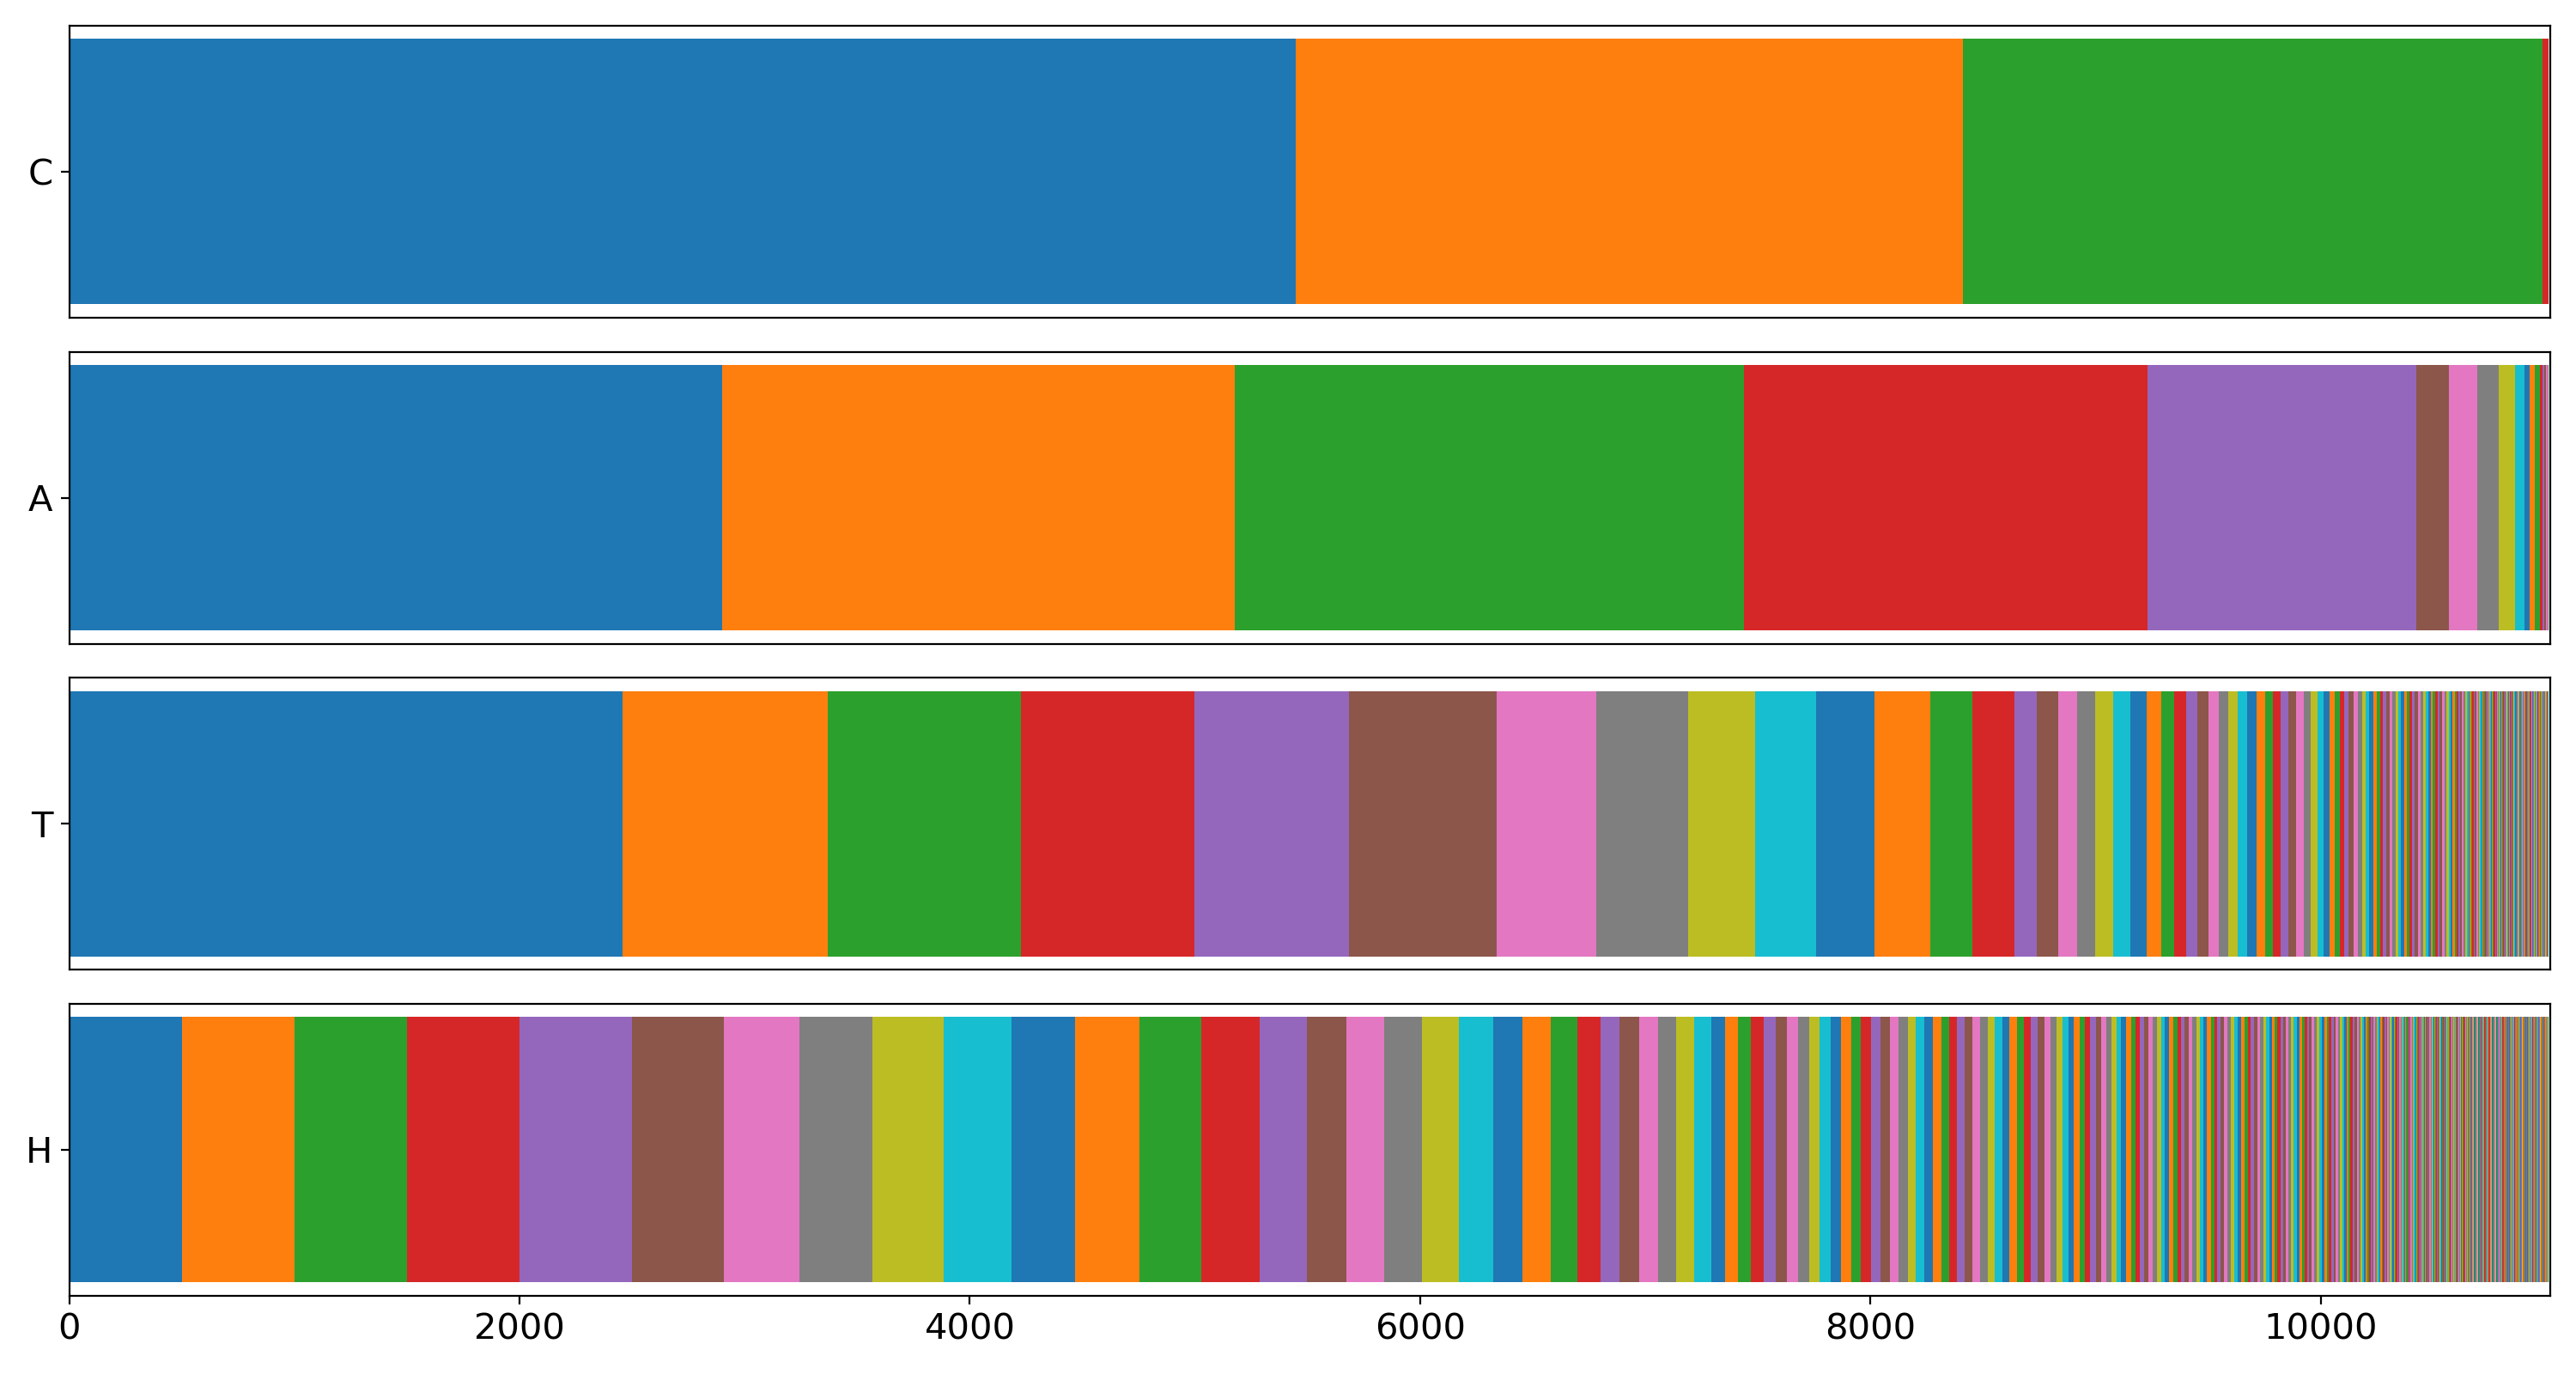
\includegraphics[width=\linewidth]{imgs_tomas/cath_distributions_filtered.png}
    \caption{CATH families distributions after filtering out over represented homologous superfamilies, removing segmentated domains and removing domains with missing pdb coordinates}
    \label{fig:cath_filtered}
\end{figure}

\subsubsection{Train/Validation/Test split}

\begin{figure}
    \centering
    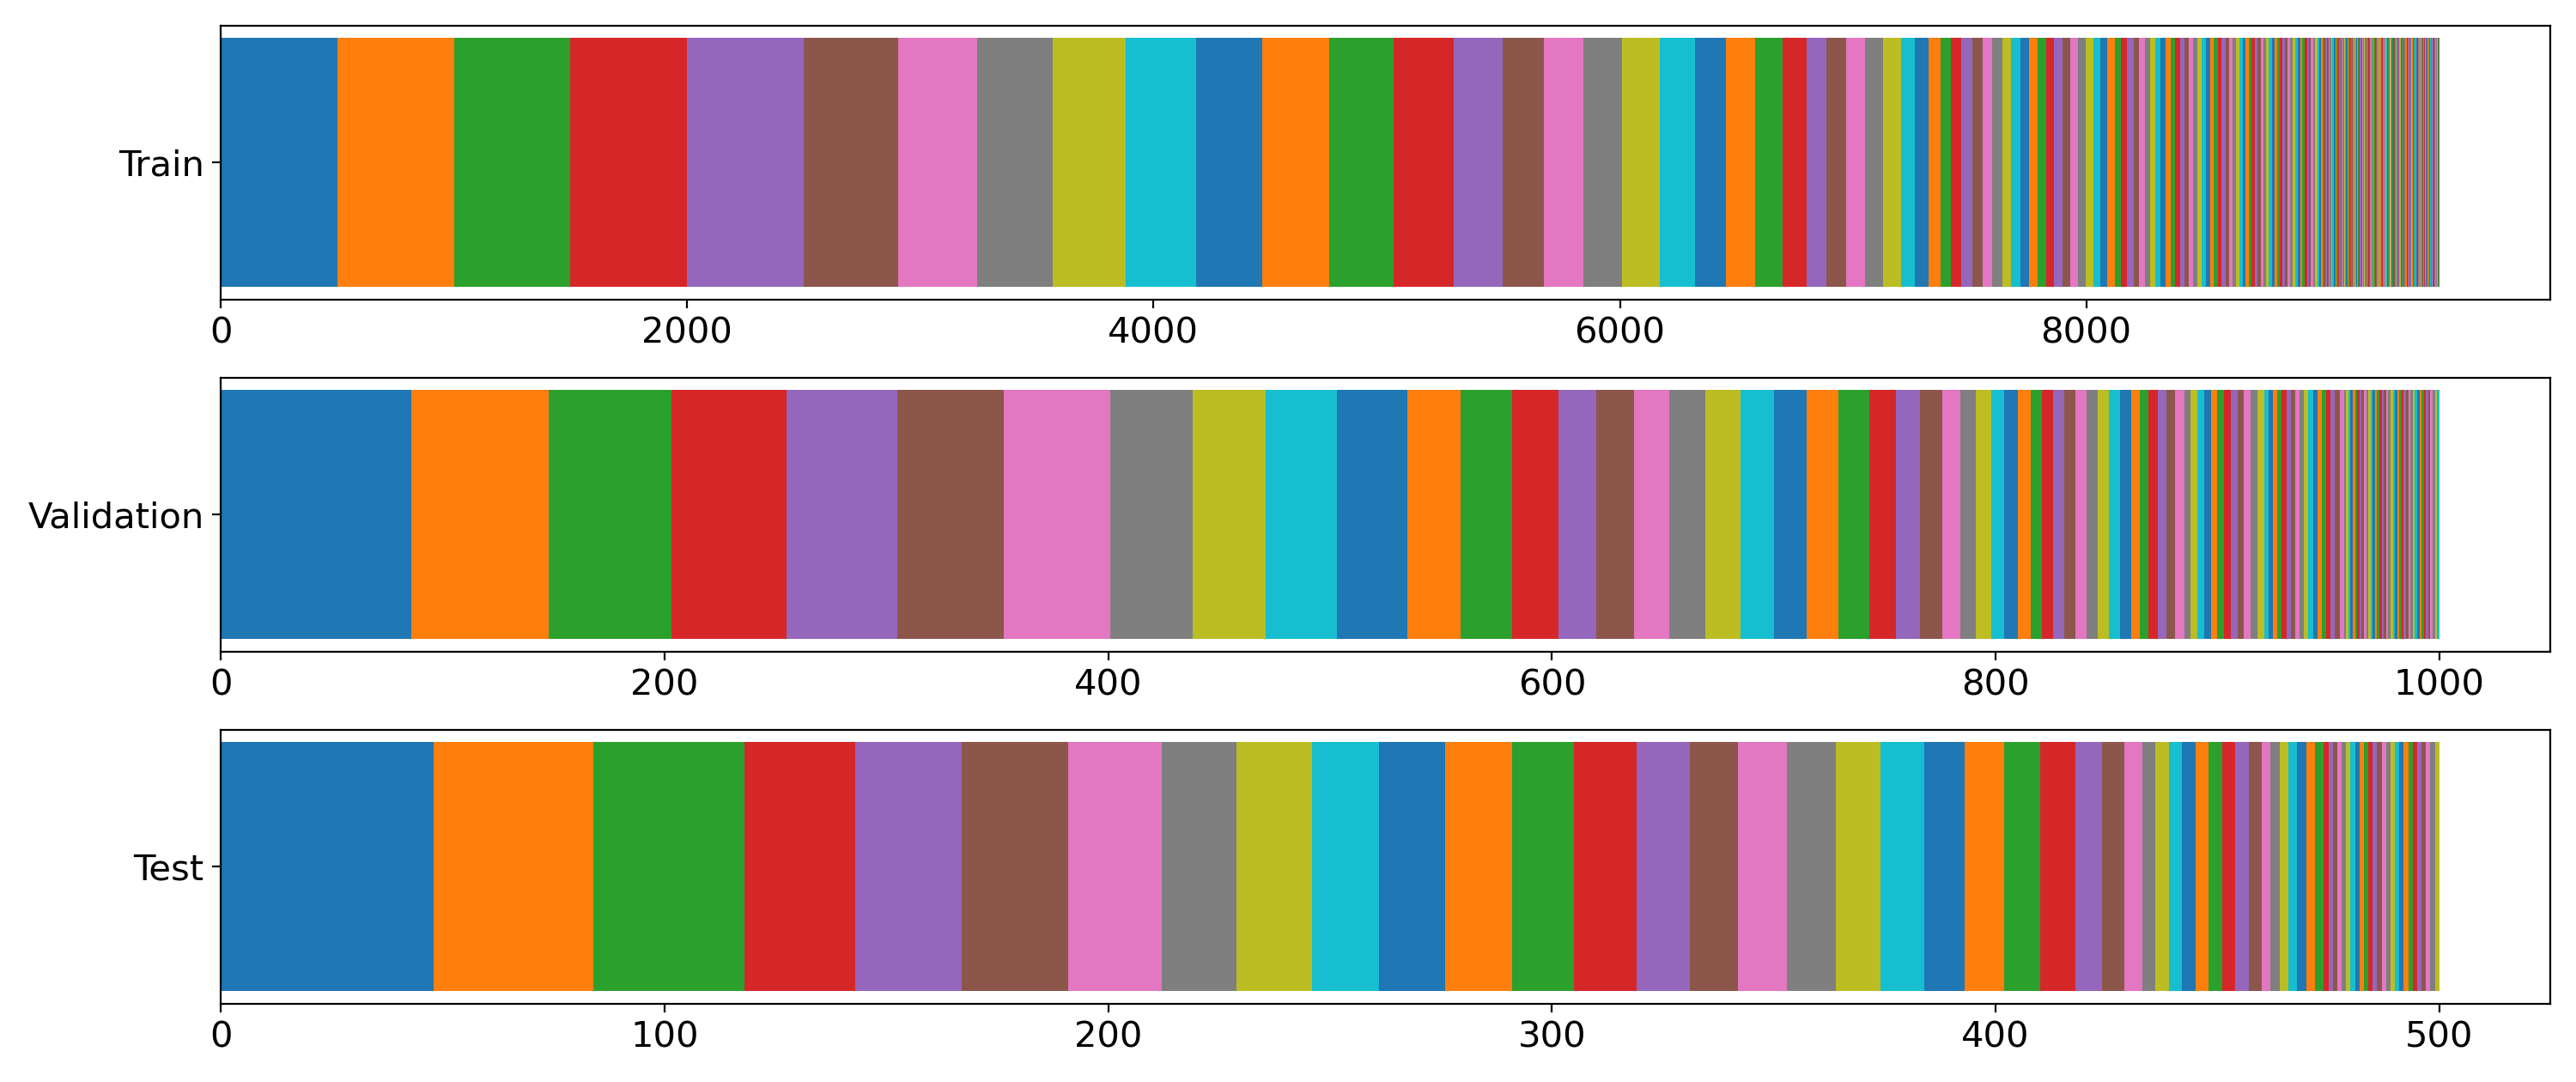
\includegraphics[width=\linewidth]{imgs_tomas/cath_distributions_trainvaltest.png}
    \caption{Represantion of homologous superfamilies in Train, Validaton and Test set. (The colors do not correspond to the same superfamilies, they simply divide the superfamilies in each row)}
    \label{fig:cath_trainvaltest}
\end{figure}

In the AlphaFold paper \cite{alphafold}, the authors decided to create train/validation/test set of homologous superfamilies instead of randomly picking the domain. 
The rationale behind this is to include all members of each homologous superfamily in either training, validation or test set. 
This ensures that when evaluating the model performance of a set of proteins, that very similar proteins were not used for training. 
    
We decided to train our models on a set of 9394 domains (several had to be excluded due to factors such as low sequence similarity to known structures or inability to converge/slow convergence of the Potts Model). This set of domains was used to train the neural networks and for the estimation of the loss during the training process.

The performance of the different models was evaluated on an independent validation set of 1000 domains. For each model we evaluated its inter-residue distance predictions as well as the auxiliary outputs (secondary structure and phi and psi torsion angles).

The final structures and performance metrics were evaluated on a set of 500 test domains.
    
Furthermore, to simulate the famous CASP competition we downloaded the domains from CASP13 (2018) - regular targets category (T). This allowed us to compare our results with the best teams in the world.